
\section{Sphere generation}
\label{sec:sphere}

\begin{frame}
    \frametitle{Sphere Particle Cluster}
    Extension of our generators \newline
    \textbf{Idea:}
    \begin{itemize}
        \item 2D Discs: Concentric rings of particles
        \item 3D Sphere: Stack of discs
        \item Trigonometric functions for even spacing of particles
    \end{itemize}
\end{frame}

\begin{frame}
    \frametitle{Trigonometric functions}
    \textbf{Angular step calculation:}
    \begin{itemize}
        \item Angular step $\theta$ between particles for spacing at least at a given distance along the circumference.
        \item Given a ring with radius \textit{r} and particle spacing \textit{s}, the angular step $\theta$ is determined by:
        \item $\theta = 2 \arcsin\left(\frac{s}{2 \times r}\right)$
    \end{itemize}
    \textbf{Number of particles calculation:}
    \begin{itemize}
        \item The number of particles \textit{N} given by dividing the full circle ($2\pi\ radians$) by the angular step $\theta$:
        \item $N = \left\lfloor \frac{2\pi}{\theta} \right\rfloor$
    \end{itemize}
    \textbf{Positioning of particles:}
    \begin{itemize}
        \item Calculation using polar coordinates, for a particle at index \textit{i}:
        \item $x_i = \text{origin}_x + r \cos(i \theta)\newline y_i = \text{origin}_y + r \sin(i \theta)\newline z_i = \text{origin}_z + \text{z\_offset}$
    \end{itemize}
\end{frame}

\begin{frame}
    \frametitle{Final Sphere}
    \begin{figure}
        \label{fig:sphere}
        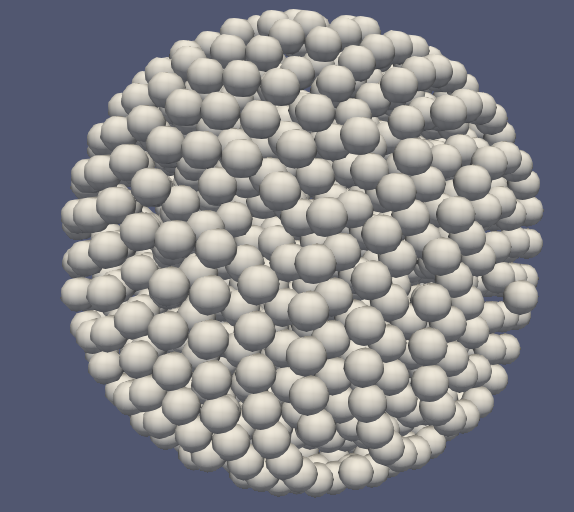
\includegraphics[width=0.5\textwidth]{../../res/sphere}
    \end{figure}
\end{frame}